\newpage
\section{Перечисление проекций $k$-танглов}
	\label{section:projections}

		Как и было сказано выше, в данной главе будет дано описание алгоритма, перечисляющего простые связные проекции
		$k$-танглов с количеством перекрестков, не превосходящим заданное число. Проекции считаются одинаковыми, если
		одну можно перевести в другую композицией плоской изотопии и элемента группы $D_{2k}$, то есть если они гомеоморфны.

	\subsection{Элементарные операции с проекциями}
		\label{subsection:cutting}

		\begin{definition}
			Перекресток проекции называется пограничным, если он соединен одним из ребер проекции с одним из ее концов.
		\end{definition}

		\begin{definition}
			Удалением пограничного перекрестка проекции называется операция, при которой выбранный перекресток
			удаляется из проекции вместе с ребрами, соединяющими его с концами проекции, а ребра, которые раньше
			соединяли удаленный перекресток с остальной частью проекции, теперь соединяют остальную часть с новыми
			концами проекции. При этом требуется, чтобы удаляемый перекресток был соединен с каким-либо другим
			перекрестком проекции. Число концов проекции может при этом меняться на $0$, $2$, или $-2$. Обратная
			операция называется приклеиванием пограничного перекрестка. 
		\end{definition}

		\begin{figure}[ht]
			\centering
			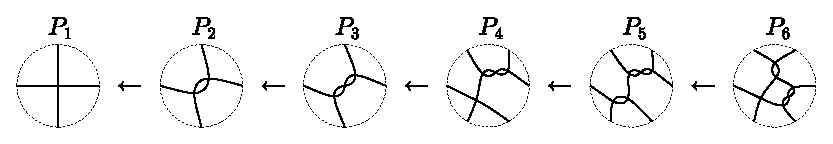
\includegraphics{c/geneology.eps}
			\caption{Последовательные удаления перекрестков\label{figure:geneology}}
		\end{figure}

		К любой проекции, удовлетворяющей нашим условиям и содержащей перекрестки, мы можем последовательно применять операцию
		удаления пограничного перекрестка как на \figureref{figure:geneology}, вопрос лишь в том, можно ли это делать так,
		чтобы в конце всегда получалась проекция из одного перекрестка, а все промежуточные проекции были просты и связны.
		Или, иными словами, любую ли простую связную простую проекцию с перекрестками можно получить из проекции, состоящей
		из одного перекрестка, последовательными приклеиваниями пограничного перекрестка так, чтобы все промежуточные проекции
		были простые и связные. Ответ здесь положительный, благодаря Теореме~\ref{theorem:good-cutting}.

		\begin{theorem}
			\label{theorem:good-cutting}
			В любой связной простой проекции $k$-тангла, содержащей более одного перекрестка, можно удалить пограничный
			перекресток так, чтобы получившаяся в результате проекция была простой и связной.
		\end{theorem}
		\begin{proof}
			Простота любой получающейся проекции очевидна. Осталось доказать возможность получения связной проекции, показав,
			что среди пограничных перекрестков найдется не являющийся точкой сочленения проекции. Точка сочленения --- перекресток,
			через которую можно провести хорду (гладкую несамопересекающуюся кривую, только начало и конец которой лежат на граничной
			окружности), которая больше нигде с проекцией не пересекается, и с обеих сторон от которой есть перекрестки.
			\begin{figure}[H]
				\centering
				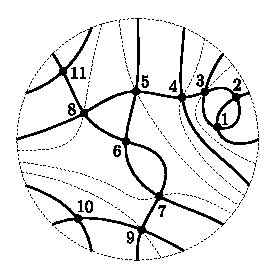
\includegraphics{c/cutpoints-proof.eps}
				\caption{К доказательству Теоремы~\ref{theorem:good-cutting}\label{figure:cutpoints-proof}}
			\end{figure}
			Проведем через все точки сочленения проекции соответствующие хорды таким образом, чтобы они все не пересекались
			(легко доказать, что так всегда можно сделать) как на \figureref{figure:cutpoints-proof}. Каждая из хорд
			делит круг на две части, и всегда за конечное число шагов найдется ``крайняя'' хорда, у которой точки сочленения
			есть только по одну сторону. Но перекрестки там есть по определению точки сочленения, значит есть и пограничные
			перекрестки, так как диаграмма простая.
		\end{proof}

		Исходя из вышеприведенных утверждений, уже можно предложить следующий алгоритм: обозначим за $P_n$ множество всех
		связных простых проекций с $n$ перекрестками, за $P_1$ возьмем множество из единственной проекции с одним перекрестком.
		Имея $P_n$, вычислим $P_{n+1}$ следующим образом: возьмем мультимножество результатов всех возможных приклеиваний
		пограничного перекрестка ко всем проекциям из $P_n$ и удалим из него дубликаты и составные проекции.

		Однако, этот алгоритм не очень хорош, так как содержит трудоемкую стадию удаления дубликатов. Ниже будет показано, как
		от нее избавится.

	\subsection{Инвариант помеченных проекций}
		\label{subsection:root-code}

		\begin{definition}
			Помеченной проекцией называется связная проекция $k$-тангла, снабженная тройкой $r = (v, e, f)$, где $v$ ---
			перекресток проекции, $e$ --- ребро проекции, инцидентное $v$ и $f$ --- грань проекции, инцидентная $v$ и $e$.
			$v$ назовем помеченным перекрестком, $e$ --- помеченным ребром и $f$ --- помеченной гранью.
		\end{definition}

		Положение грани $f$ относительно перекрестка $v$ и ребра $e$ задает направление обхода, которое может быть по часовой
		стрелки и против часовой стрелки.

		Построим теперь инвариант помеченной $(v, e, f)$ проекции $P$ (который мы назовем ``root-code'') следующим образом
		(см. Алгоритм~\ref{algorithm:root-code} и \figureref{figure:rcode-example}):

		\begin{algorithm}[H]
			\caption{root-code$(P, (v, e, f))$\label{algorithm:root-code}}
			\algsetup{linenosize=\small, linenodelimiter=.}
			\begin{algorithmic}[1]
				\STATE $A \leftarrow \{\}$
				\STATE $free \leftarrow 2$

				\STATE $Q \leftarrow \{v\}$
				\STATE $number[v] \leftarrow 1$
				\STATE $incoming[v] \leftarrow e$

				\WHILE{$Q \neq \varnothing$}
					\STATE $u \leftarrow head[Q]$
					\STATE $dequeue(Q)$

					\FOR{(для) всех ребер $(u, w) \in P$ в порядке, заданном $f$, начиная с $incoming[u]$}
						\IF{$w$ --- конец диаграммы}
							\STATE $code \leftarrow 0$
						\ELSE
							\IF{$number[w]$ не определен}
								\STATE $number[w] \leftarrow free$
								\STATE $free \leftarrow free + 1$
								\STATE $enqueue(Q, w)$
							\ENDIF
							\STATE $code \leftarrow number[w]$
						\ENDIF

						\STATE $push(A, code)$
					\ENDFOR
				\ENDWHILE

				\RETURN $A$
			\end{algorithmic}
		\end{algorithm}

		\begin{figure}[ht]
			\centering
			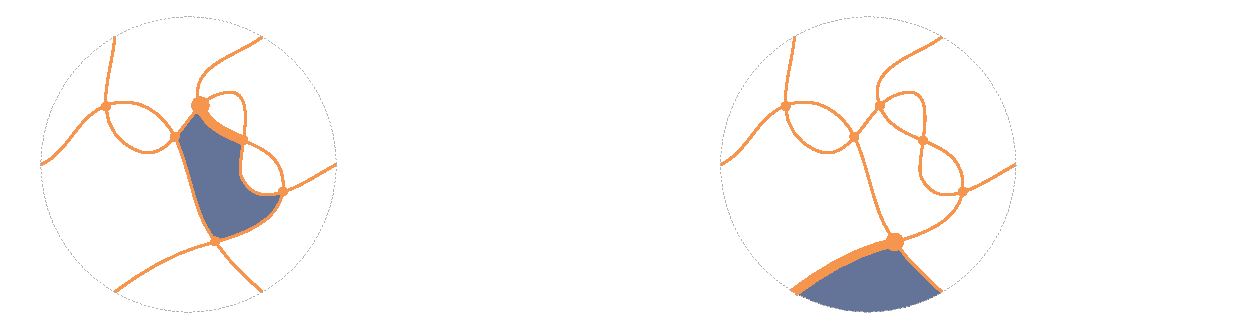
\includegraphics{c/rcode-example.eps}
			\caption{Примеры вычисления root-code\label{figure:rcode-example}}
		\end{figure}

		Результатом работы алгоритма будет последовательность, в которой на каждый перекресток проекции $P$ приходится по 4 числа ---
		номера соседних перекрестков в порядке обхода, заданном гранью $f$, или $0$, если данный сосед является концом диаграммы.
		Номера присваиваются перекресткам начиная с единицы в порядке обхода в ширину. В инварианте вершины описаны также в порядке
		возрастания номера.

		Легко понять, что по такому инварианту и направлению обхода исходная проекция однозначно восстанавливается, следовательно
		это и правда инвариант помеченных проекций. Определим теперь root-code($P$, $v$) перекрестка $v$ проекции $P$ как
		лексикографически минимальный root-code среди всех восьми способов пометить проекцию $P$ с помеченной вершиной $v$. Заметим,
		что root-code($P$, $v$) = root-code($P$, $u$) для $v \neq u; v, u \in P$ тогда и только тогда, когда существует автоморфизм
		(гомеоморфизм на себя) проеции $P$, переводящий $v$ в $u$.

	\subsection{Алгоритм}

		\begin{figure}[ht]
			\centering
			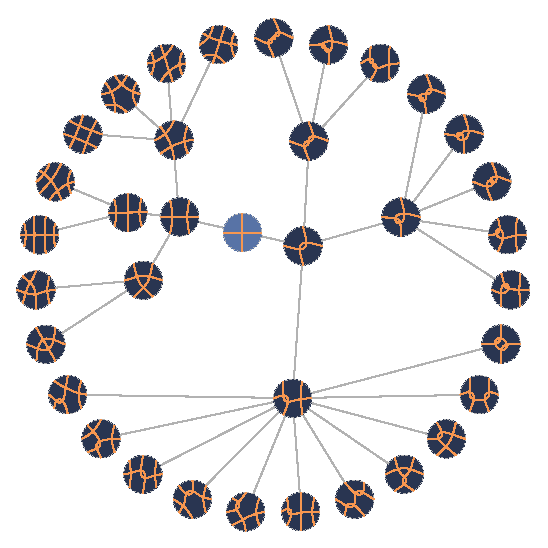
\includegraphics{c/genealogical-tree.eps}
			\caption{Дерево проекций\label{figure:genealogical-tree}}
		\end{figure}

		\begin{definition}
			Пусть $I$ --- проекция тангла, состоящая из единственного пререкрестка. Определим на множестве простых связных
			прекций $k$-танглов отображение $prev(T)$ следующим образом:
			\begin{itemize}
				\item
				$prev(I) = \varnothing$

				\item
				Для всех остальных $prev(T)$ будет являться результатом удаления из $T$ пограничного перекрестка $v$, не
				являющегося точкой сочленения, такого что root-code($T$, $v$) лексикографически минимален среди всех подобных
				перекрестков.
			\end{itemize}
		\end{definition}

		Согласно результатам параграфа~\ref{subsection:cutting}, отображение $prev(T)$ определено на всем множестве простых связных
		проекций $k$-танглов. Оно однозначно благодаря тому, что все удовлетворяющие определению способы выбора перекрестка отличаются
		друг от друга автоморфизмом (см. параграф~\ref{subsection:root-code}), следовательно все результаты удаления таких пограничных
		перекрестков гомеоморфны друг другу, а гомеоморфные проекции мы друг от друга не отличаем. И, наконец, оно обладает
		полуинвариантом --- числом перекрестков. Благодаря всем перечисленным свойствам, $prev(T)$ задает на множестве всех связных
		простых проекций структуру бесконечного дерева с корнем в $I$ (см.~\figureref{figure:genealogical-tree}).

		Таким образом, для перечисления всех проекций не более чем с $n$ перекрестками достаточно обойти это дерево DFS-ом на глубину
		не более, чем $n$ (см.~Алгоритм~\ref{algorithm:projections-enumeration}). Единственный тонкий момент, который мы должны
		учитывать --- это не спускаться по одному и тому же ребру несколько раз.

		\begin{algorithm}[ht]
			\caption{DFS(T)\label{algorithm:projections-enumeration}}
			\algsetup{linenosize=\small, linenodelimiter=.}
			\begin{algorithmic}[1]
				\PRINT $T$
				\IF{$crossings[T] = n$}
					\RETURN
				\ENDIF

				\STATE $list \leftarrow \varnothing$
				\FOR{(для) всех возможных результатов $R$ приклеивания перекрестка $v$ к $T$}
					\IF{$R$ --- простая}
						\IF{$prev(R) = T$}
							\STATE $r \leftarrow $ root-code($R$, $v$)
							\IF{ {\bf not} $contains(list, r)$}
								\STATE DFS($R$)
								\STATE $add(list, r)$
							\ENDIF
						\ENDIF
					\ENDIF
				\ENDFOR
			\end{algorithmic}
		\end{algorithm}

	\subsection{Результаты}

		Количества проекций $k$-танглов не более чем с 12 перекрестками, полученные в результате выполнения алгоритма, приведены
		в Таблице~\ref{table:tangle-projections}.

		\begin{landscape}
		\begin{table}[ht]
			\caption{Количество проекций $k$-танглов с $n$ перекрестками.\label{table:tangle-projections}}
			\centering
			\begin{tabular}{|c||r|r|r|r|r|r|r|r|r|r|r|r|}
			\hline
			$k$\textbackslash $n$
			    & 1 & 2 & 3 &  4 &   5 &   6 &      7 &       8 &        9 &          10 &           11 &            12 \\
			\hline\hline
			2   & 1 & 1 & 2 &  6 &  19 &  71 &    293 &  1\,348 &   6\,568 &     33\,701 &     178\,706 &      973\,085 \\
			3   & . & 1 & 2 &  8 &  29 & 138 &    638 &  3\,237 &  16\,805 &     90\,239 &     494\,151 &   2\,756\,453 \\
			4   & . & . & 2 &  8 &  41 & 210 & 1\,125 &  6\,138 &  34\,112 &    192\,278 &  1\,096\,560 &   6\,317\,363 \\
			5   & . & . & . &  5 &  31 & 231 & 1\,458 &  9\,183 &  56\,084 &    340\,885 &  2\,060\,224 &  12\,446\,400 \\
			6   & . & . & . &  . &  16 & 161 & 1\,406 & 10\,572 &  74\,331 &    499\,902 &  3\,276\,104 &  21\,112\,641 \\
			7   & . & . & . &  . &   . &  60 &    840 &  8\,818 &  75\,747 &    591\,091 &  4\,327\,816 &  30\,451\,898 \\
			8   & . & . & . &  . &   . &   . &    261 &  4\,702 &  56\,199 &    541\,570 &  4\,628\,641 &  36\,633\,417 \\
			9   & . & . & . &  . &   . &   . &      . &  1\,243 &  26\,753 &    361\,106 &  3\,846\,580 &  35\,758\,786 \\
			10  & . & . & . &  . &   . &   . &      . &       . &   6\,257 &    155\,593 &  2\,332\,512 &  27\,199\,662 \\
			11  & . & . & . &  . &   . &   . &      . &       . &        . &     32\,721 &     916\,595 &  15\,123\,600 \\
			12  & . & . & . &  . &   . &   . &      . &       . &        . &           . &     175\,760 &   5\,464\,661 \\
			13  & . & . & . &  . &   . &   . &      . &       . &        . &           . &            . &      963\,900 \\
			\hline
			все & 1 & 2 & 6 & 27 & 136 & 871 & 6\,021 & 45\,241 & 352\,856 & 2\,839\,086 & 23\,333\,649 & 195\,201\,866 \\
			\hline
			\end{tabular}
		\end{table}
		\end{landscape}
